\chapter{Implementación}

En este capítulo comentaremos a fondo las decisiones tomadas que hemos comentado previamente en base a la especificación, además de describir las implementaciones propuestas con las distintas tecnologías utilizadas. Pondremos el foco no solo en el \textbf{software implícito en el robot} sino también a los componentes desarrollados externos a él, pero que también conforman la arquitectura completa de la plataforma, como lo son el \textbf{sistema operativo}, el \textbf{panel web de administración} y otras herramientas involucradas. Las ideas que por una razón u otra no hayan llegado a implementarse a tiempo, serán definidas en profundidad en apartados posteriores.\\

Para elaborar este capítulo de una forma más legible y entendible, seguiremos una estructura muy similar a la propuesta en el capítulo 3 de \textbf{Especificación de requisitos}.\\


\section{Requisitos generales}


\subsection{Licencias y compartición del software}

En cuanto a licencias y permisos del proyecto, como se anticipó se usarán diversos \textbf{repositorios} en \textit{Github}, que aparecen listados a continuación y descritos en función del contenido (que se elaborará más tarde):

\begin{itemize}
	\item \textbf{\textit{lazarillo-embedded}} \cite{lazarillo-embedded}: se trata del software embebido programado en \textbf{\textit{C++}} que da lógica al robot.
	\item \textbf{\textit{lazarillo-admin-frontend}} \cite{lazarillo-admin-frontend}: es la página web que utilizan los técnicos para supervisar los robots y enviarles determinadas acciones. Se encuentra hecho en \textbf{\textit{React}} y utiliza \textit{WebSockets} para la conexión con el dispositivo.
	\item \textbf{\textit{lazarillo-admin-backend}} \cite{lazarillo-admin-backend}: es un servicio web que actúa como intermediario entre el robot y el servicio de \textbf{\textit{frontend}} para la negociación de la conexión. Está programado en \textbf{\textit{Python}} usando la librería de \textbf{\textit{Flask}} principalmente.
	\item \textbf{\textit{meta-lazarillo}} \cite{meta-lazarillo}: aquí se aloja el \textit{layer} (o ``capa'') personalizada para \textit{The Yocto Project} con la que se especifican las dependencias de \textbf{\textit{Lazarillo}} en la compilación del sistema operativo del robot.
	\item \textbf{\textit{documentacion-tfm}} \cite{documentacion-tfm}: en este repositorio se alojan los fuentes de \textbf{\LaTeX} para generar esta misma documentación que se está leyendo.
\end{itemize}

Todos los repositorios listados se publican bajo la licencia \textbf{\textit{GPL}} en su \textit{versión 3} (cuya última declaración es del 29 de junio de 2007 \cite{gplv3}) y que permite a cualquier interesado utilizar el software e incluso ampliar sus funcionalidades mientras que posteriormente se distribuya con la misma licencia.

Habiendo establecido ésto, entremos en materia y veamos todos los detalles de la implementación.\\


\section{Sistema operativo}

Como comentábamos en el capítulo del \textit{Estado del arte} en el apartado de \textit{Sistema operativo, el cerebro del robot}, existen diversas alternativas para componerlo. Partiendo de la base de que contamos con una \textit{Raspberry} como núcleo del computador, las opciones más sonadas son utilizar \textit{\textbf{Raspbian}} (sistema ya compilado e instalable en la plataforma) o crear nuestra propia distribución utilizando \textbf{el proyecto \textit{Yocto}}.\\

¿Por qué omitimos un sistema operativo que ya existe? Pues bien, la respuesta es fácil. \textit{Raspbian} es un sistema operativo de uso general que permite utilizar la \textit{Raspberry} como cualquier ordenador normal, ya sea para ofimática, desarrollo de software, consumo de recursos multimedia o incluso videojuegos. Esto provoca que el sistema operativo en cuestión venga con demasiado \textit{bloatware} (software innecesario que no se utiliza) preinstalado de base; y llevaría más tiempo modificar la imagen de \textit{Raspbian} para que no contenga todo el software no deseado que confeccionar un sistema operativo a medida. Además, deseamos que el robot solo muestre una aplicación embebida en pantalla en lugar de un entorno de escritorio normal, por lo que podemos prescindir de este entorno completo y configurar nuestro nuevo sistema para que solo muestre una aplicación y ahorre tiempo en el arranque.\\

La ventaja de crear nuestra propia imagen de sistema permitirá que incluyamos solo las librerías y dependencias que realmente necesitemos, obviando aspectos que no nos sea necesario incluir y que tomarían un espacio útil en la máquina. Además, siendo un proyecto de código abierto permitirá que interesados aprovechen el sistema operativo y lo extiendan con las funcionalidades y programas que les apetezca. Pasemos a continuación a comentar la implementación realizada.\\

\textbf{Nota}: este documento no se pretende que sea una guía de cómo utilizar \textit{Yocto} y entender todo su ecosistema, por lo que solo destacaremos las configuraciones personalizadas hechas para darle forma a \textbf{\textit{lazarillo-image}}.\\

Para empezar a trabajar con \textit{Yocto}, lo primero es elegir \textbf{la versión de \textit{Yocto}} a utilizar y seguir su documentación oficial sobre \textit{Quick Build} \cite{yocto-quick-build}, en la que se detalla cómo clonar el proyecto y realizar una primera compilación de prueba. Esta ejecución inicial llevará al menos un par de horas, ya que necesitará descargar todas las librerías necesarias y compilarlas.\\

\begin{figure}[h]
	\centering
	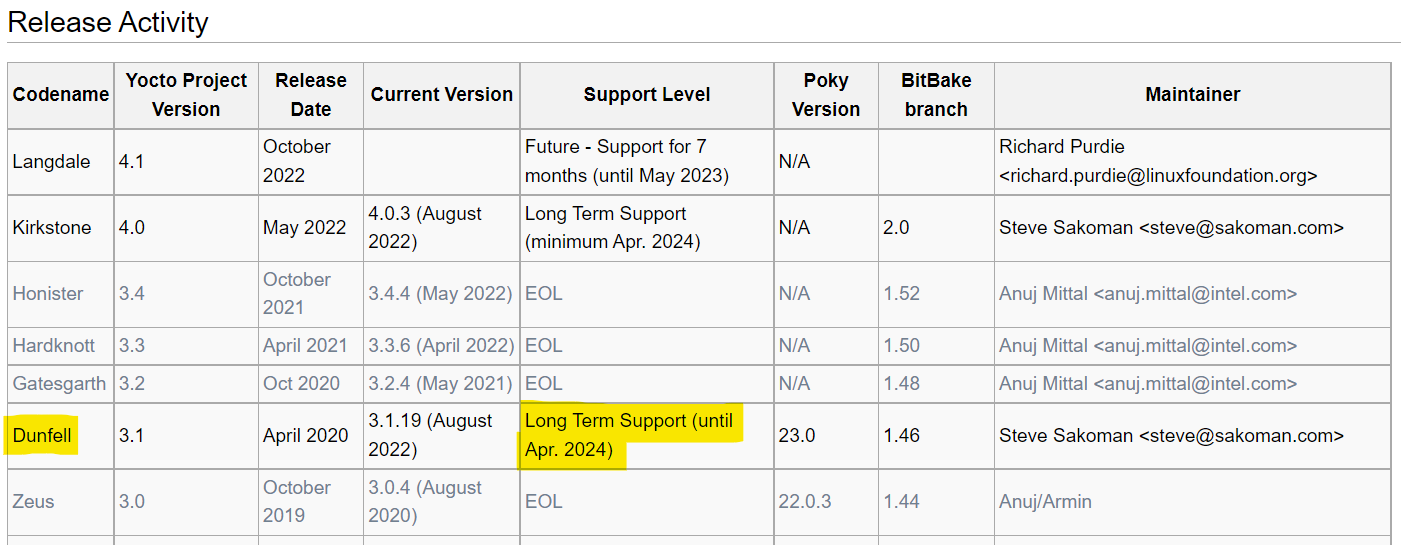
\includegraphics[width=0.85\textwidth]{imagenes/yocto-releases.png}
	\caption{La versión elegida es \textbf{\textit{Dunfell 3.1}} ya que lleva el suficiente tiempo en el mercado como para ser estable, y además es versión \textit{Long Term Support} y asegura soporte oficial hasta abril de 2024. Versiones más novedosas o no \textit{LTS} pueden no asegurar tanta estabilidad. - Fuente: \textit{Yocto Releases} \cite{yocto-releases}}
	\label{yocto-releases}
\end{figure}

Acto seguido, lo que hacemos para continuar con la creación de nuestra propia distribución son varias cosas:

\begin{itemize}
	\item Crear nuestro propio \textit{layer}, llamado \textbf{\textit{meta-lazarillo}} donde estableceremos nuestras directivas.
	\item Crear una \textbf{imagen} de sistema, que se llamará \textbf{\textit{lazarillo-image}} y que incluirá el software programado por nosotros y que se instalará automáticamente en el robot.
	\item Añadir a la imagen creada previamente las dependencias para que sus aplicaciones se ejecuten correctamente.
\end{itemize}

El contenido de este \textit{layer} puede verse en la web \cite{meta-lazarillo} pero igualmente listaremos aquí los archivos más representativos.\\

\subsubsection{conf/layer.conf}

Este primer archivo contiene las variables más genéricas para la configuración inicial del \textit{layer} y suele tener un formato parecido en todos los \textit{metas} que se crean, ya que principalmente fija el nombre característico de la colección además de la rama de \textbf{compatibilidad} (que es \textit{dunfell}) como hemos comentado arriba. 

\begin{lstlisting}
BBPATH .= ":${LAYERDIR}"

BBFILES += "${LAYERDIR}/recipes-*/*/*.bb \
${LAYERDIR}/recipes-*/*/*.bbappend"

BBFILE_COLLECTIONS += "lazarillo"
BBFILE_PATTERN_lazarillo = "^${LAYERDIR}/"
BBFILE_PRIORITY_lazarillo = "1"

LAYERSERIES_COMPAT_lazarillo = "dunfell"
LAYERVERSION_lazarillo = "1"
\end{lstlisting}


\subsubsection{recipes-core/images/lazarillo-image.bb}

A continuación, veamos el archivo que realmente define \textbf{la imagen} del sistema operativo, cuyo nombre utilizaremos cuando queramos compilarlo.

\begin{lstlisting}
inherit core-image lazarillo-class

GLIBC_GENERATE_LOCALES = "es_ES.UTF-8"

###################################################
# Groups of needed packages

CORE_PKGS = " \
	kernel-devicetree \
	kernel-image \
	kernel-modules \
	openssl \
"

MISC_PKGS = " \
	curl \
	nano \
	psplash \
"

QT_PKGS = " \
	qtbase qtbase-plugins qtbase-tools \
	qtdeclarative qtdeclarative-qmlplugins \
	qtgraphicaleffects qtgraphicaleffects-qmlplugins \
	qtmultimedia qtmultimedia qtmultimedia-plugins qtmultimedia-qmlplugins \
	qtquickcontrols qtquickcontrols-qmlplugins \
	qtquickcontrols2 qtquickcontrols2-qmlplugins \
	qtvirtualkeyboard qtvirtualkeyboard-plugins qtvirtualkeyboard-qmlplugins \
"

LAZARILLO_PKGS = " \
	lazarillo-embedded \
"

###################################################
# Installation of grouped packages

IMAGE_FEATURES += " \
	autologin \
"

IMAGE_INSTALL += " \
	${CORE_PKGS} \
	${MISC_PKGS} \
	${QT_PKGS} \
	${LAZARILLO_PKGS} \
"
\end{lstlisting}

Todas las constantes del tipo \emph{X\_PKGS} tan solo son valores auxiliares que se concatenan a \emph{IMAGE\_INSTALL} para que en la compilación se incluyan todas estas dependencias en el sistema de ficheros final.\\

Si nos fijamos en el valor de \emph{LAZARILLO\_PKGS} podemos ver que ahí se lista \textbf{lazarillo-embedded}, que se trata de la aplicación embebida que comentábamos que implementará toda nuestra lógica del robot. Vemos el contenido de su \textbf{receta} (como se llaman en \textit{Yocto} los archivos que definen cómo se debe obtener una pieza de software, compilarla e instalarla en el destino) en el siguiente apartado.\\


\subsubsection{recipes-core/lazarillo-embedded/lazarillo-embedded.bb}

\begin{lstlisting}
# Compiles Qt project with cmake after downloading
inherit cmake_qt5

# AUTOREV references to newest commit
SRCREV = "${AUTOREV}"
LICENSE = "GPLv3"

EXTRA_OECMAKE = "-DCOMPILE_MODE=d"

# Reference to repo where to download the software from
SRC_URI = "git://git@github.com/adrianmorente/lazarillo_hmi.git;protocol=ssh"

DEPENDS += " \
	qtbase \
	qtdeclarative \
	qtgraphicaleffects \
	qtmultimedia \
	qtquickcontrols \
	qtquickcontrols2 \
	qtvirtualkeyboard \
"

do_install() {
	install -d ${D}${bindir}
	install -m 0700 lazarillo-hmi ${D}${bindir}
	install -m 0700 motor-manager ${D}${bindir}
	install -m 0700 web-gateway ${D}${bindir}
}

FILES_${PN} = "${bindir}"
\end{lstlisting}

En el archivo mostrado se configura la \textit{URL} del repositorio del que \textit{Yocto} descargará el proyecto (usando las claves \textit{SSH} configuradas en el dispositivo de compilación).\\

Además, encontramos listadas las dependencias necesarias para la compilación exitosa del proyecto. Como utilizamos el framework \textit{Qt} en su versión \textbf{open source} (disponible en \cite{qt-open-source}) para construir la aplicación embebida, se enumeran las librerías que \textit{Yocto} deberá descargar e instalar también.\\

Para finalizar, con \emph{do\_install} establecemos que se copien al directorio normal de binarios del sistema operativo final (normalmente \emph{/usr/bin}) los tres programas generados por \emph{lazarillo-embedded}, con permisos de escritura, lectura y ejecución solo para el usuario actual. Por ahora nos ceñiremos a lo estrictamente relacionado con \textit{Yocto} y estos servicios los definiremos en detalle más adelante.\\


\subsubsection{Configuración local y compilación}

Una vez que tenemos nuestro \textit{layer} preparado para que \textbf{\textit{bitbake}}, la herramienta en \textit{Python} que gestiona las compilaciones de \textit{Yocto}, pueda encontrar nuestros paquetes y dependencias, pasamos a configurar el archivo \emph{build/conf/local.conf}, que es el realmente imprescindible. En este archivo podríamos haber añadido todo el contenido de configuración necesaria para compilar nuestra imagen, si bien es mucho más limpio utilizar \textit{layers} separados que poder versionar y controlar de forma independiente según la \textit{release} de \textit{Yocto} que queramos usar.\\

El contenido usado para el archivo es el siguiente (se han obviado algunas líneas por defecto de \textit{Yocto} que solo son para desarrollo y que no aportan mucho para el alcance de este documento):

\begin{lstlisting}
MACHINE = "raspberrypi3"

DISTRO = "poky"
DISTRO_FEATURES_append = " alsa alsa-plugins gles2 opengl pulseaudio systemd wifi"
DISTRO_FEATURES_REMOVE_append = " x11 wayland"
PACKAGECONFIG_pulseaudio += " systemd"
VIRTUAL-RUNTIME_init_manager = "systemd"
DISTRO_FEATURES_BACKFILL_CONSIDERED = "sysvinit"

PACKAGE_CLASSES = "package_deb"

BB_NUMBER_THREADS = "4"
PARALLEL_MAKE = "-j 4"

EXTRA_USERS_PARAMS += " usermod -a -G audio root;"
EXTRA_USERS_PARAMS += " usermod -P lazarillo123 root;"

EXTRA_IMAGE_FEATURES ?= "debug-tweaks"
\end{lstlisting}


En primer lugar, fijamos la \emph{MACHINE} de destino para la que queremos compilar, en este caso la \textit{Raspberry Pi 3} como hemos comentado anteriormente. Además, decimos a \textit{Yocto} que genere nuestra imagen de sistema operativo utilizando \emph{poky} como distribución base (que es la \textit{de facto} en la herramienta), además de añadir paquetes como \textit{Alsa}, \textit{Pulseaudio}, \textit{OpenGL} y \textit{Systemd}.\\

\begin{itemize}
	\item \textit{Alsa} y \textit{Pulseaudio} son dependencias para los sistemas de sonido, que aunque no se utilizan actualmente, se incluyen en el sistema para cuando se quieran emitir alertas sonoras a través del servicio \textbf{lazarillo-hmi} y así proporcionar una interfaz más cercana y accesible para los usuarios del robot.
	\item \textit{OpenGL} (y su complemento \textit{GLES2}) se incluyen ya que son requisitos indispensables para que el framework de \textit{Qt} con aplicaciones de interfaz gráfica funcione como esperamos en dispositivos embebidos. Gracias a esto, utilizamos el lenguaje \textit{QML} del framework (basado en \textit{Javascript}) para diseñar dicha aplicación con interfaz táctil.
	\item \textit{Systemd} se establece en el sistema como gestor de servicios y \textbf{demonios} (o \textit{daemons}, pequeños servicios que se ejecutan en segundo plano en el sistema). Este es el gestor de arranque de servicios por defecto en la mayoría de distribuciones modernas que utilizamos hoy en día para escritorio.
\end{itemize}

Para terminar, fijamos a \textit{Bitbake} que utilice 4 hilos en la compilación. Cuantos más se utilicen, más tareas de descarga/compilación/instalación podrán ejecutarse en paralelo. Obviamente dependerá de la máquina utilizada.\\

Para terminar, añadimos una contraseña al usuario \textit{root} por defecto para que no se pueda manipular libremente el robot por consola si se accede por \textit{ssh}.\\

Una vez tenemos listo nuestro \textit{layer} y el archivo \textit{local.conf}, podemos lanzar la orden \textbf{\textit{bitbake lazarillo-image}} en el directorio de desarrollo de \textit{Yocto} y ver cómo comienza a descargar dependencias y compilarlas en la arquitectura de la \textit{RPi}:

\begin{figure}[h]
	\centering
	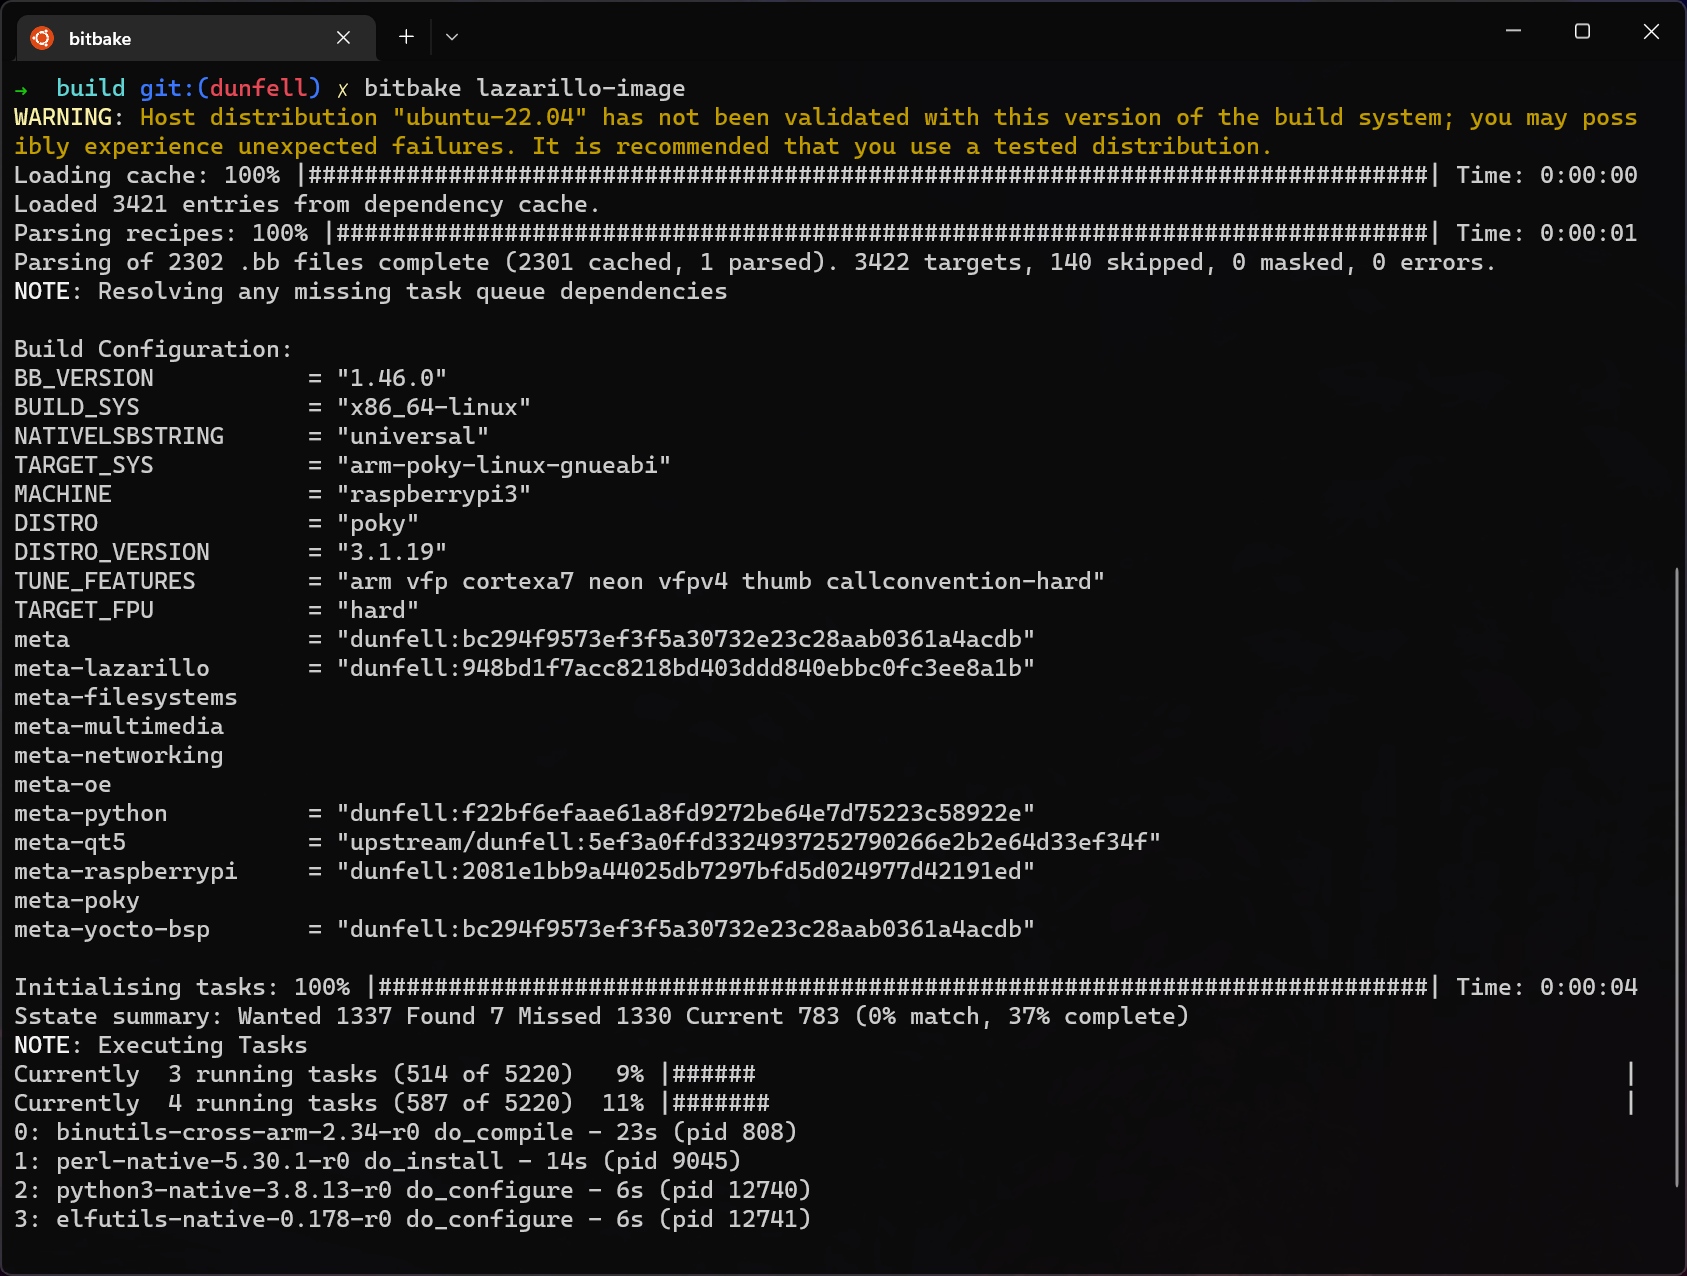
\includegraphics[width=0.95\textwidth]{imagenes/lazarillo-image-compilation.png}
	\caption{Captura de pantalla de \textit{Ubuntu 22.04} sobre el Subsistema Linux de Windows, usado para la compilación del nuevo sistema operativo.}
	\label{lazarillo-image-compilation}
\end{figure}

Llegados aquí, solo quedará esperar unas horas a que termine todo el proceso. Una vez finalizado, grabaremos el archivo \textbf{\textit{lazarillo-image-raspberrypi3.sdimg}} generado bajo el directorio \emph{build/tmp/deploy/} en la tarjeta de memoria que queramos usar en el robot, la insertamos en la \textit{Raspberry} correspondiente y probamos nuestro nuevo y flamante sistema operativo personalizado.\\


\subsubsection{Personalización del sistema operativo}

Para cerrar con el sistema operativo, comentemos el caso de \textbf{\textit{psplash}} \cite{psplash}, un programa que se instala en \textbf{lazarillo-image.bb} dentro del grupo \emph{MISC\_PKGS} como dependencia externa y que permite mostrar una imagen estática durante el arranque del dispositivo final.\\

Detalles como éste hacen que el dispositivo tenga un aspecto más profesional, dado que en lugar de mostrarse una imagen genérica de \textit{GNU/Linux} o, peor si cabe, una terminal de arranque; el robot mostraría en su pantalla una imagen customizada (que podría ser un logo personalizado del proyecto, si lo hubiera).\\

Basta con integrar esta sencilla aplicación dentro del sistema operativo, cambiar la imagen que se desea mostrar y (re)compilar el sistema operativo. Sin embargo, por falta de tiempo, no he podido generar un logo personalizado para el proyecto que mostrar, por lo que el logo por defecto de \textit{OpenEmbedded} es el mostrado al iniciar.\\

\begin{figure}[h]
	\centering
	
\includegraphics[width=0.3\textwidth]{imagenes/openembedded.jpg}
	\caption{Imagen mostrada por \textit{psplash} al arranque de la máquina: logo de \textit{OpenEmbedded}, organización contribuidora activamente en el Proyecto \textit{Yocto} - Fuente: \textit{OpenEmbedded.org} \cite{openembedded}}
	\label{openembedded}
\end{figure}


\section{Arquitectura de Lazarillo}

Una vez que hemos visto la integración completa del sistema operativo, en esta sección enumeraremos los distintos servicios y módulos específicos creados para \textit{Lazarillo} y describiremos el propósito para el que han sido programados. Como venimos comentando, habrá ciertas partes que serán enteramente embebidas en el robot, y por otro lado también existirán otros componentes software que estarán situados ``fuera''.\\

Una idea que se ha tenido muy presente durante el desarrollo del proyecto es la de cumplir los famosos \textbf{principios \textit{SOLID}} de la programación orientada a objetos. Véase en el capítulo de \textit{Estado del arte} cuáles son cada uno de los puntos.\\

Para cumplir esto, se implementan módulos separados de \textbf{responsabilidad única}, lo que resulta en clases no muy grandes y fácilmente mantenibles con un propósito muy claro y que colaboran entre sí. Además, se utilizan interfaces generales que permiten luego a las clases derivadas gestionar su comportamiento más concreto.\\

Se persigue una arquitectura que carezca de \textbf{acoplamiento} y el uso de interfaces ayuda a que ciertos componentes software sean luego intercambiables y no estrictamente dependientes. Por ejemplo: si se desea no utilizar \textit{Redis} para la mensajería interna y se intercambia por \textit{MQTT}, este cambio solo se realiza en el módulo \textbf{\textit{messaging-broker}} y resulta totalmente transparente al resto de servicios, que directamente heredan ese comportamiento.\\

Para hacernos una idea general de todos los entes involucrados en el software, prestemos atención al diagrama de la figura \ref{lazarillo-architecture}.\\

\begin{figure}[h]
	\centering
	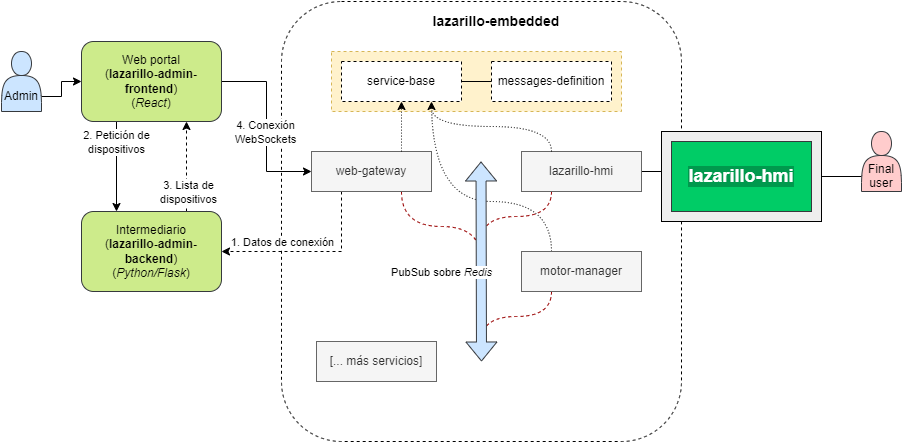
\includegraphics[width=\textwidth]{imagenes/lazarillo-architecture.png}
	\caption{Diagrama mostrando la arquitectura del proyecto, incluyendo conexiones entre servicios y relaciones internas.}
	\label{lazarillo-architecture}
\end{figure}

A la izquierda del todo, junto al agente denominado \textit{Admin} se ubican los dos servicios web involucrados que ya hemos mencionado (\textbf{lazarillo-admin}, arriba \textbf{frontend} y \textbf{backend} abajo). A su derecha encontramos un rectángulo grande que engloba todo el software enclaustrado (\textbf{lazarillo-embedded}) y para finalizar, la interfaz de usuario (gráfica táctil y sonora) con la que interactuarán los que necesiten de la atención de \textit{Lazarillo}.\\

Para explicar la implementación, separaremos todo el software en tres módulos: uno para el software embebido y otro por cada servicio web (que son dos). Aunque ya venimos anunciando cosas, entraremos a continuación en detalles más profundos de lenguajes de programación y librerías utilizadas.\\


\subsection{lazarillo-embedded}

Si volvemos a mirar el diagrama \ref{lazarillo-architecture}, distinguimos el cuadrado blanco que incluye los módulos presentes en \textit{lazarillo-embedded}. Por un lado tenemos los comprendidos en el rectángulo blanco que se tratan de \textbf{librerías}, las cuales se enlazan al compilar a los \textbf{servicios}, representados por rectángulos grises (y comunicados sobre el búfer de comunicación en azul). En esta sección describiremos la razón de existencia de cada uno y el propósito que persiguen, empezando por las librerías y acabando por los programas que se ejecutan en el robot.\\

Hagamos un pequeño inciso aquí para comentar que la compilación está gestionada con la herramienta \textit{CMake} \cite{cmake}, una opción escalable y muy útil para proyectos grandes. Permite establecer funciones y macros comunes para todos los componentes involucrados dentro de un proyecto, utilizando variables para customizar la compilación. Además, con el uso de \emph{cpack} también permite generar archivos \emph{.deb} entendibles por el sistema operativo para su posterior instalación.\\

Antes de nada, veamos la estructura del proyecto hasta el primer nivel de directorios, sin entrar en cada uno, definiendo cada uno de ellos así como los ficheros presentes y la utilidad de cada uno, aunque algunos con más enjundia se desarrollarán más tarde:\\

\textbf{NOTA:} los directorios se muestran en negrita cursiva y los archivos solo en cursiva.

\begin{itemize}
	\item \textit{\textbf{cmake/}ProjectSetup.cmake}: contiene el código común de \textit{CMake} para la correcta compilación del proyecto. Define las banderas de compilación, rutas donde localizar las librerías necesarias e implementa funciones y macros que utilizarán los servicios para enlazarse con las librerías de las que dependen (\textit{Qt}, \textit{Json}, \textit{Redis} y \textit{Systemd}).
	\item \textit{\textbf{lazarillo-hmi/}}: subproyecto que implementa la aplicación gráfica mostrada en la pantalla táctil del robot.
	\item \textit{\textbf{lazarillo-utils/}}: librería que añade objetos estáticos accesibles para todos los subproyectos. En esta fase solo contiene métodos estáticos para obtener la fecha y hora del sistema y así proveerla de forma estándar a los servicios.
	\item \textit{\textbf{messages-definition/}}: este módulo no es en sí un servicio que se ejecute directamente en el sistema operativo sino una \textbf{librería} de la que se nutren los demás donde se definen los mensajes que utilizan internamente para comunicarse. Ésta a su vez se enlaza con el servicio que describiremos más tarde y cuyo fin es \textbf{serializar} los mensajes.
	\item \textit{\textbf{messaging-broker/}}: esta librería es la que establece toda la comunicación con el servidor de \textit{Redis} para el manejo de \textbf{mensajería sobre \textit{PubSub}}. Contiene clases para gestionar la conexión y utiliza el patrón de diseño \textit{Factory} para la creación de los objetos que publican mensajes y se suscriben a tópicos. Al gestionar la conexión en solo este módulo, si se decidiera cambiar \textit{Redis} por otra alternativa, al ser un comportamiento heredado para los servicios, el cambio debería ser solo un trámite.
	\item \textit{\textbf{motor-manager/}}: idealmente, este directorio contiene un nuevo servicio llamado \textit{motor-manager} cuya idea es la de \textbf{controlar los distintos motores y elementos electrónicos que permiten que el robot se mueva}. Contendría clases distintas por cada elemento conectado e intercambiaría mensajes con todos ellos. Desafortunadamente, \textbf{no ha llegado a implementarse} ninguna funcionalidad en esta fase del proyecto.
	\item \textit{\textbf{serialization/}}: esta librería contiene los tipos de datos para \textbf{serialización} (y deserialización) utilizando el formato \textit{Json}. Realmente se podría prescindir de este módulo y almacenar todos los mensajes como texto plano sobre \textit{Redis} y enviarlos así a los servicios. Lo que permite la serialización es transformar los datos para almacenarlos en un búfer (o cualquier recipiente) y que luego puedan ser reconstruidos en el mismo o en otro dispositivo. Se sigue esta aproximación (\textit{por si acaso}) simplemente por dotar de algo más de escalabilidad al proyecto por si sigue creciendo y se quieren hacer más cosas con los mensajes.
	\item \textit{\textbf{service-base/}}: aunque el nombre pueda inducir a pensar que se trate de un \textit{servicio}, realmente es una librería que incluye interfaces y clases que reutilizarán todos los servicios que quieran crearse posteriormente. Realiza acciones generales interesantes como \textbf{instanciar el bróker de mensajería} (mencionado arriba) y proveer de métodos que se ejecutarán tanto al inicio como al final del resto de programas directamente.
	\item \textit{\textbf{test\_env/}}: si bien esta parte no ha llegado a probarse profusamente, el objetivo que persigue es el de crear un entorno de pruebas para el desarrollo en forma de contenedores de \textit{Docker}. Con un archivo \emph{docker-compose.yml} se levantan dos instancias de éstos, uno que simula los servicios instalados en el robot y otro que mantiene el servidor de \textit{Redis} donde se realiza la comunicación. Usando esto, es posible \textbf{probar el código del robot en nuestra máquina local}, ahorrando tiempo.
	\item \textit{\textbf{web-gateway/}}: esta sencilla aplicación hace de \textit{gateway} entre el robot y el panel externo de administración. Mantiene un servidor \textit{WebSocket} que recibe los comandos de la web, los procesa y traduce a mensajes (de \textit{messages-definition}) que luego publica en \textit{Redis} para que las aplicaciones interesadas y suscritas los reciban. De esta forma, un administrador que usa el panel web puede enviar distintas órdenes.
	\item \textit{.clang-format}: ésto no es más que una recomendación a desarrolladores. Si bien este archivo no aporta funcionalidad como tal al proyecto, sí que lo hace al desarrollo. \textit{ClangFormat} \cite{clang-format} se trata de una herramienta que permite dar formato automático al código conforme se escribe. Si se configura este archivo con el editor de texto y las variables siguiendo las \textbf{guías de estilo} que se acuerden con el equipo de desarrollo, todos los programadores involucrados podrán trabajar sobre un estilo común. Ésto evitará conflictos con el control de versiones cuando alguien inserta espacios sin percatarse o más saltos de línea de la cuenta.
	\item \textit{build.sh}: este archivo es un \textbf{\textit{script}} realmente útil para el desarrollo. Internamente ejecuta los comandos de \textit{CMake} con sus parámetros necesarios, permitiendo customizar el proceso con argumentos simples como \emph{-j8} para utilizar 8 hilos en la compilación, \emph{-c d} para compilar en modo de depuración o \emph{--cpack} para generar los binarios de instalación si la compilación es exitosa. Véase la imagen \ref{lazarillo-build-sh}.
	\item \textit{CMakeLists.txt}: finalmente, este es el archivo central del proyecto. Simplemente utiliza el código de la carpeta \textbf{\textit{cmake/}} para incluir el comportamiento general allí descrito y añade a la compilación cada uno de los módulos (exactamente las librerías y los servicios que ya hemos listado).
\end{itemize}

\begin{figure}[h]
	\centering
	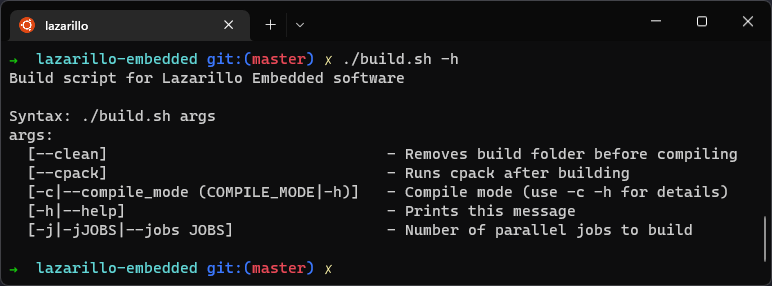
\includegraphics[width=0.6\textwidth]{imagenes/lazarillo-build-sh.png}
	\caption{Captura de pantalla del uso del script \emph{build.sh} para compilación de \textit{lazarillo-embedded}.}
	\label{lazarillo-build-sh}
\end{figure}

A partir de ahora, veremos el código más relevante para entender la lógica del proyecto. Por temas de espacio, se obviarán del código las guardas, los \textit{namespaces} y los comentarios, además de incluir la implementación de los métodos (ubicados en los archivos \emph{*.cpp} en lugar de \emph{*.h} como de costumbre). Si se quieren ver los archivos completos, véase el enlace del título de cada fragmento.\\

\subsubsection{messages-definition}

En el punto de implementación alcanzado a la hora de la entrega del proyecto no existen muchos mensajes, pero la librería se ha pensado de forma que sea sencillo añadir mensajes nuevos para los nuevos desarrolladores que quieran participar en ello y utilizar \textit{Lazarillo}.\\

Para ilustrar este comportamiento, veremos dos clases: una \textbf{interfaz genérica} para todos los mensajes y una \textbf{clase objeto} de ejemplo que la implementa. Empecemos por la interfaz:\\

\textbf{\textit{\href{https://github.com/adrianmorente/lazarillo-embedded/blob/master/messages-definition/inc/messages-definition/i_base_message.h}{i\_base\_message.h}}}
\begin{lstlisting}
class IBaseMessage : public serialization::Serializable
{
public:
	~IBaseMessage() {}

	virtual std::string name() const = 0;

	void setHeader(MessageHeader const &p_header)
	{
		m_header = std::make_shared<MessageHeader>(p_header);
	}

	MessageHeader getHeader() const
	{
		return (m_header) ? *m_header : getDefaultHeader();
	}

	MessageHeader getDefaultHeader() const;
	{
		MessageHeader header;
		header.name = name();
		return header;
	}

	virtual serialization::Serializer & serializePayload(serialization::Serializer &p_serializer) const = 0;

	serialization::Serializer & serialize(serialization::Serializer &p_serializer) const override
	{
		return serializePayload(p_serializer);
	}
	
private:
	std::shared_ptr<MessageHeader> m_header;
};
\end{lstlisting}

Vemos que esta clase abstracta hereda de \emph{serialization::Serializable}, presente en el módulo de \textbf{serialization} y que provee los métodos que han de sobreescribirse para añadir los campos al objeto serializado que se guardará en memoria.\\

El mensaje abstracto utiliza una \textit{MessageHeader} que compone la \textbf{cabecera} que heredarán todos los mensajes. Tiene tres campos:

\begin{itemize}
	\item \textbf{name}: nombre del mensaje en cuestión, a cumplimentar por cada clase que herede de \textit{IBaseMessage}.
	\item \textbf{source}: nombre del servicio que lo envía.
	\item \textbf{timestamp}: fecha y hora en la que se compone el mensaje para su envío.
\end{itemize}

Además de proveer métodos de acceso para la cabecera, declara los métodos de serialización y deserialización que implementarán cada una de las clases hijas. Un detalle a considerar en éstos es que reciben y devuelven referencias al objeto de serialización; esto se hace para poder concatenar los campos en una sola línea. Ejemplo:

\begin{lstlisting}
# Sin usar referencias como argumento y retorno:	
p_serializer.add("campo1");	
p_serializer.add("campo2");	
p_serializer.add("campo3");
return p_serializer;

# Usando referencias:
return p_serializer.add("campo1").add("campo2").add("campo3");
\end{lstlisting}

Veamos ahora un ejemplo de mensaje que implemente dicha interfaz. Usaremos la clase \textit{EventConnectionStatus}, que representa el mensaje que se envía del servicio \textbf{web-gateway} al resto de servicios cuando cambia la conexión por \textit{WebSocket} con el portal de administración:\\

\textbf{\textit{\href{https://github.com/adrianmorente/lazarillo-embedded/blob/master/messages-definition/inc/messages-definition/event_connection_status.h}{event\_connection\_status.h}}}
\begin{lstlisting}
class EventConnectionStatus : public IBaseMessage
{
public:
	static constexpr char const *NAME{"EVENT_CONNECTION_STATUS"};
	
	explicit EventConnectionStatus(models::ConnectionStatus p_status)
	: m_status{p_status} {}
	
	explicit EventConnectionStatus(serialization::Deserializer &p_deserializer)
	{
		p_deserializer.extract("Status", m_status);
	}
	
	serialization::Serializer & serializePayload(serialization::Serializer &p_serializer) const final
	{
		IBaseMessage::serializePayload(p_serializer);
		return p_serializer.add("Status", m_status);
	}
	
	std::string name() const final { return NAME; }
	
private:
	models::ConnectionStatus m_status{models::ConnectionStatus::UNKNOWN};
};
\end{lstlisting}

Podemos ver que utilizando esta aproximación, el código necesario para crear un nuevo mensaje es bastante sencillo. Simplemente sobreescribe el nombre con el que se identificará y especifica qué campos han de añadirse o leerse. La variable que se utiliza en cuestión (\emph{m\_status}) no es más que un enumerado con los posibles estados de la conexión (\emph{UNKNOWN}, \emph{CONNECTED}, \emph{NOT\_CONNECTED}).


\subsubsection{service-base}

Este módulo define el esqueleto abstracto de cada uno de los servicios del robot. Heredando el comportamiento de esta librería, cada uno de los nuevos servicios se ahorran procedimientos rutinarios como instanciar la conexión con la base de datos y el bróker de mensajería.\\

Solamente contiene dos interfaces que aprovecharán el resto de módulos. Comentémoslas a continuación:\\

\textbf{\textit{\href{https://github.com/adrianmorente/lazarillo-embedded/blob/master/service-base/inc/service-base/service_base.h}{service\_messager.h}}}
\begin{lstlisting}
class ServiceMessager
{
public:
	ServiceMessager(std::shared_ptr<lzr::msg::Broker> p_broker, std::shared_ptr<messages::MessageFactory> p_message_factory, std::string const &p_service_name)
	{
		auto serialization = std::make_shared<lzr::msg::serialization::SerializationFactory>();
		m_pub = lzr::msg::createMsgPublisher(p_broker, serialization, p_service_name);
		m_sub = lzr::msg::createMsgSubscriber(p_broker, serialization, p_message_factory);
	}
	
	bool publish(std::string const &p_topic, messages::IBaseMessage const &p_message)
	{
		return m_pub->publish(p_topic, p_message);
	}

	void subscribe(std::string const &p_topic, std::string const &p_message, std::shared_ptr<lzr::msg::IBaseMessageReceiver> p_receiver)
	{
		m_sub->subscribe(p_topic);
		m_sub->add_receiver(p_message, p_receiver);
	}
	
	auto get_pub() const { return m_pub; }
	auto get_sub() const { return m_sub; }
	
private:
	std::shared_ptr<lzr::msg::MsgPublisher> m_pub;
	std::shared_ptr<lzr::msg::MsgSubscriber> m_sub;
};
\end{lstlisting}

Esta es una clase auxiliar para \textit{ServiceBase} que envuelve las utilidades para publicar y suscribirse a mensajes fácilmente desde cualquier servicio. Utiliza dos objetos: \textit{MsgPublisher} y \textit{MsgSubscriber} que enlaza del módulo \textbf{messaging-broker} y que permite gestionar de forma sencilla la mensajería.\\

El método para \textbf{publicar} (\textit{publish}) hace lo que se espera: simplemente enviar el mensaje. Sin embargo, el método \textbf{\textit{subscribe}}, además de suscribir el servicio correspondiente al tópico y mensaje de \textit{PubSub} especificado, asocia un \textit{callback} que será llamado cuando se publique dicho mensaje. Este \textbf{\textit{IBaseMessageReceiver}} es otra interfaz de \textit{messaging-broker} que define el comportamiento general de lo que se ha bautizado como \textit{message receivers}, y que simplemente implementan la lógica ejecutada cuando se recibe el mensaje esperado.\\

\textbf{\textit{\href{https://github.com/adrianmorente/lazarillo-embedded/blob/master/service-base/inc/service-base/service_messager.h}{service\_base.h}}}
\begin{lstlisting}
class ServiceBase
{
public:
	virtual std::string get_name() = 0;
	virtual void init() = 0;
	virtual int run_internal() = 0;
	virtual void finish() = 0;
	
	int run()
	{
		// Abstract initialisation for communication
		init_messaging();
		
		// Initialisation steps given by child class
		init();
		
		std::cout << "Running service " << get_name() << std::endl;
		sd_notify(0, "READY=1");
		
		auto exit_code = run_internal();
		
		std::cout << "Stopping service " << get_name() << std::endl;
		sd_notify(0, "STOPPED=1");
		
		return exit_code;
	}

	bool publish(std::string const &p_topic, messages::IBaseMessage const &p_message)
	{
		return m_messager->publish(p_topic, p_message);
	}

	void subscribe(std::string const &p_topic, std::string const &p_message, std::shared_ptr<msg::IBaseMessageReceiver> p_receiver)
	{
		m_messager->subscribe(p_topic, p_message, p_receiver);
	}
	
private:
	void init_messaging()
	{
		auto broker = std::shared_ptr<lzr::msg::Broker>();
		
		constexpr auto CONNECTION_TIMEOUT{5s};
		auto const connected = broker->connect_async(CONNECTION_TIMEOUT).get();
		if (!connected)
		{
			throw std::runtime_error("Unable to connect to broker.");
		}
		
		auto message_factory = std::make_shared<messages::MessageFactory>();
		
		m_messager = std::make_shared<lzr::service::ServiceMessager>(broker, message_factory, get_name());
	}
	
	std::shared_ptr<ServiceMessager> m_messager;
};
\end{lstlisting}

En esta clase abstracta \textit{ServiceBase} ocurre todo el comportamiento genérico que utilizamos en los servicios que realmente se ejecutan en el robot. Si miramos el método \textbf{\textit{run()}} distinguimos los siguientes pasos:

\begin{itemize}
	\item \textbf{init\_messaging()}: es un método privado que intenta realizar la conexión con el bróker de mensajería y compone los objetos de publicación/suscripción utilizando una \textbf{fábrica}, siguiendo el patrón de diseño \textbf{\textit{Factory Method}} \cite{factory-method}. Éste facilita la creación de objetos concretos a partir de una interfaz común.
	\item \textbf{init()}: se trata de un método virtual que implementan las clases hijas para definir todo el comportamiento de inicialización que necesiten sus servicios.
	\item Llamadas a \textbf{sd\_notify(...)}: es una función de la librería de \textit{Systemd} y se utiliza para avisar al sistema operativo del estado actual del servicio en cuestión.
	\item \textbf{run\_internal}: otro método virtual para que los servicios herederos implementen el \textit{loop} de su funcionamiento real. 
\end{itemize}

Llegados aquí, pasemos al fin a ver uno de los servicios que se ejecutan en el robot, concretamente el que se muestra en la pantalla táctil con la que puede interactuar el usuario.\\


\subsubsection{lazarillo-hmi}

Se trata de la aplicación que muestra la interfaz táctil al usuario. La tecnología usada por esta aplicación ha sido el framework de \textbf{\textit{Qt}}, que pese a tener modalidades de licencias de pago, permite un uso \textit{open source} \cite{qt-open-source}. Además, se trata de una tecnología con una amplia comunidad, una documentación muy rica y un gran soporte para dispositivos embebidos. De hecho, \textit{Qt} distribuye sus propios \textit{layers} para poder utilizarlos en \textit{Yocto} y así descargar automáticamente las librerías necesarias para nuestra aplicación.\\

Por otro lado, dispongo de amplia experiencia con dicha herramienta, lo que agiliza enormemente el tiempo de desarrollo. Utilizamos la versión \textbf{5.15.5} de la herramienta, versión \textit{LTS} y última de la versión \textit{major} número \textbf{5}. Si bien me habría gustado utilizar la \textbf{6}, que es la más novedosa y ya está en el mercado, me habría supuesto tener que ponerme a estudiar sobre ella y analizar todas las diferencias, lo cual requería un tiempo que no tenía.\\

El \textit{framework} se compone a su vez de las librerías para \emph{C++} y un lenguaje para implementación de interfaces gráficas basado en \textit{JavaScript}, llamado \textbf{\textit{QML}}. Se puede obtener más información en su página web \cite{qt-qml}.

Empecemos viendo el archivo \emph{CMakeLists.txt} con el que se describe lo necesario para poder compilar el servicio:\\

\textbf{\textit{\href{https://github.com/adrianmorente/lazarillo-embedded/blob/master/lazarillo-hmi/CMakeLists.txt}{CMakeLists.txt}}}
\begin{lstlisting}
project(lazarillo-hmi VERSION 0.1 LANGUAGES CXX)

set(_include_dir inc/lazarillo-hmi)
set(TS_FILES i18n/lazarillo-hmi_es_ES.ts)

set(PROJECT_SOURCES
	${_include_dir}/utils/style.h
	${_include_dir}/service.h
	src/message_receivers/event_reboot_receiver.cpp
	src/message_receivers/event_reboot_receiver.h  
	src/utils/style.cpp
	src/main.cpp
	src/service.cpp
	gui/qml.qrc
	gui/img.qrc
	${TS_FILES}
)

add_executable(${PROJECT_NAME} ${PROJECT_SOURCES})

lzr_link_qt(${PROJECT_NAME})
lzr_link_systemd(${PROJECT_NAME})

qt5_create_translation(QM_FILES ${CMAKE_SOURCE_DIR} ${TS_FILES})

target_include_directories(${PROJECT_NAME} PUBLIC inc)
target_include_directories(${PROJECT_NAME} PRIVATE src)

target_link_libraries(${PROJECT_NAME} PRIVATE
	messages-definition
	messaging-broker
	serialization
	service-base
)
\end{lstlisting}

En la variable \emph{PROJECT\_SOURCES} se enumeran todos los ficheros fuente necesarios para el proyecto, tanto de \textit{C++} como de \textit{QML} (incluidos en ficheros del tipo \emph{.qrc}), que luego se pasan como parámetro a \emph{add\_executable} para generar el binario de ejecución.\\

Las funciones \emph{lzr\_link\_qt} y \emph{lzr\_link\_systemd} utilizan el archivo \href{https://github.com/adrianmorente/lazarillo-embedded/blob/master/cmake/ProjectSetup.cmake}{cmake/ProjectSetup.cmake} para enlazar con las librerías de \textit{Qt} y \textit{Systemd}, de forma similar a lo que se hace en \emph{target\_link\_libraries} pero con los módulos internos del proyecto.\\

Pasemos ahora a ver código de la parte lógica en \textit{C++} y la interfaz gráfica en \textit{QML}. Empezaremos por ver el código que inicializa el servicio y lanza la interfaz, aprovechando para ilustrar sobre el uso de la clase abstracta \textbf{\textit{ServiceBase}} explicado previamente:\\

\textbf{\textit{\href{https://github.com/adrianmorente/lazarillo-embedded/blob/master/lazarillo-hmi/inc/lazarillo-hmi/service.h}{service.h}}}
\begin{lstlisting}
class Service : public lzr::service::ServiceBase
{
public:
	Service(int argc, char *argv[])
	{
		m_app = new QGuiApplication(argc, argv);
		m_app->setOrganizationName("Adrian Morente");

		QTranslator translator;
		const QStringList uiLanguages = QLocale::system().uiLanguages();
		for (const QString &locale : uiLanguages)
		{
			if (translator.load(":/i18n/" + "lazarillo-hmi_" + QLocale(locale).name()))
			{
				m_app->installTranslator(&translator);
				break;
			}
		}
		
		qmlRegisterUncreatableType<Style>("lazarillo.utils", 1, 0, "Style", "Style enum type not creatable.");
		qRegisterMetaType<const Style *>("const Style");
	}

	~Service() { delete m_app; }
	
	std::string get_name() override { return "lazarillo-hmi"; }
	
	void init() override
	{
		auto event_reboot_receiver = std::make_shared<lzr::hmi::EventRebootReceiver>();
		subscribe(WEB_GATEWAY_EVENT_TOPIC, messages::EventReboot::NAME, event_reboot_receiver);
	}
	
	int run_internal() override
	{
		QQmlApplicationEngine engine;
		engine.addImportPath(":/");
		
		Style style;
		style.changeSkin();
		engine.rootContext()->setContextProperty("style", &style);
		
		// Finally create QML window
		const QUrl url(QStringLiteral("qrc:/main.qml"));
		QObject::connect( &engine, &QQmlApplicationEngine::objectCreated, m_app,
			[url](QObject *obj, const QUrl &objUrl)
			{
				if (!obj && url == objUrl)
				QCoreApplication::exit(-1);
			}, Qt::QueuedConnection);
		engine.load(url);
		
		return m_app->exec();
	}

private:
	QGuiApplication *m_app;
};
\end{lstlisting}

Esta clase \textit{Service} instancia un objeto del tipo \textit{QGuiApplication}, que es uno de los que provee \textit{Qt} para utilizar aplicaciones mostradas en una ventana. En el constructor inicializa la aplicación, instala los archivos de traducciones (para poder mostrar la aplicación embebida en distintos idiomas), y expone el tipo \emph{Style} de C++ a QML para poder ser usado allí.\\

El método \emph{get\_name()} informa al servicio abstracto sobre el nombre de esta aplicación (que se usa en la interfaz para mostrar \textit{logs} así como para el envío de mensajes a \textit{PubSub}).\\

En \emph{init\_internal()}, método sobreescrito de la interfaz, se inicializa el \textbf{\textit{receptor de mensaje}} para \emph{EventReboot}. Como hemos explicado antes, estos receptores implementan un comportamiento específico que se ejecuta cuando se recibe el mensaje esperado en el tópico suscrito. En este caso, este receptor simplemente reinicia el dispositivo, lo que puede ser interesante realizar desde el portal web.\\

Y para terminar, \emph{run\_internal()} implementa el método abstracto que vimos en \textbf{\textit{service-base}} que se llama en el \textit{loop} del servicio. Lo que hace es cargar un motor de QML con el código situado en \emph{main.qml} (que implementa la interfaz), asignarlo al objeto \emph{m\_app} visto antes y lanzar la aplicación.\\

Utilizando así el servicio base, el programa \textit{main} de todos los servicios queda tan limpio como se ve a continuación:\\

\textbf{\textit{\href{https://github.com/adrianmorente/lazarillo-embedded/blob/master/lazarillo-hmi/src/main.cpp}{main.cpp}}} 
\begin{lstlisting}
#include "lazarillo-hmi/service.h"

int main(int argc, char *argv[])
{
	lzr::hmi::Service service(argc, argv);
	return service.run();
}
\end{lstlisting}

Simplemente carga el objeto \emph{Service} visto arriba y llama al método \emph{run()} de la clase heredada para aprovechar la inicialización de la mensajería.\\

Para terminar con los servicios embebidos en el robot, veamos ahora el que provee el servidor \textit{WebSocket} al que se conecta el portal web.\\

\subsubsection{web-gateway}

Este servicio es el \textit{puerto de entrada} a \textit{Lazarillo} para la comunicación con el exterior. Como hemos dicho reiteradamente, realiza la comunicación mediante \textit{WebSockets} con \textbf{\textit{lazarillo-admin-frontend}} habilitando un servidor al efecto, el portal web a través del cual un técnico puede administrar los distintos robots. Actúa como intérprete de los mensajes provenientes del \textit{socket} y los publica en la mensajería interna del robot (basada en \textit{Redis}) para informar al resto de servicios de cualquier acción emitida por el servidor.\\

Además, como la comunicación basada en \textit{WebSockets} es bidireccional y el canal siempre se mantiene activo, puede enviar mensajes al servidor en cualquier momento.\\

Dado que el fichero \textbf{\textit{\href{https://github.com/adrianmorente/lazarillo-embedded/blob/master/web-gateway/CMakeLists.txt}{CMakeLists.txt}}} de este módulo sigue una estructura igual al de \textbf{\textit{lazarillo-hmi}} cambiando solo el nombre del proyecto y los ficheros fuente incluidos, nos ahorraremos la explicación, ya que no veremos nada nuevo.\\

En cuanto al archivo \textbf{\textit{\href{https://github.com/adrianmorente/lazarillo-embedded/blob/master/web-gateway/src/main.cpp}{main.cpp}}} que se ejecuta por defecto en el servicio, el código también es igual al de \textit{lazarillo-hmi}, con la salvedad de que esta vez la clase \emph{Service} (utilizada para sobreescribir la de \emph{IBaseService}) es la implementación realizada por \textit{web-gateway}. La única diferencia con respecto al servicio anterior reside en la inicialización, y es que al ser una aplicación sin interfaz gráfica que solo se ejecuta en segundo plano esperando solicitudes, solamente instancia un objeto del tipo propio \textbf{\textit{WebsocketServer}}. Veamos dicha clase:\\

\textbf{\textit{\href{https://github.com/adrianmorente/lazarillo-embedded/blob/master/web-gateway/inc/web-gateway.h}{websocket\_server.h}}}
\begin{lstlisting}
class WebsocketServer : public QObject
{
	Q_OBJECT
	
public:
	explicit WebsocketServer(const int p_port  = 8080, QObject *p_parent = nullptr)
		: QObject{p_parent}, m_socket(new QWebSocketServer(QStringLiteral("Lazarillo WS Server"),
		QWebSocketServer::NonSecureMode, this))
	{
		if (m_socket->listen(QHostAddress::Any, p_port))
		{
			qDebug() << "Listening on port: " << p_port;
			
			connect(m_socket, &QWebSocketServer::newConnection, this, &WebsocketServer::onNewConnection);
			connect(m_socket, &QWebSocketServer::closed, this, &WebsocketServer::closed);
		}
	}
	
private slots:
	void onNewConnection()
	{
		QWebSocket *client = m_socket->nextPendingConnection();
		
		connect(client, &QWebSocket::textMessageReceived, this, &WebsocketServer::processTextMessage);
		connect(client, &QWebSocket::binaryMessageReceived, this, &WebsocketServer::processBinaryMessage);
		connect(client, &QWebSocket::disconnected, this, &WebsocketServer::socketDisconnected);
		
		qDebug() << "Client connected.";
		client->sendTextMessage(QString::fromUtf8("Connection accepted from Websocket server"));
	}

	void processTextMessage(QString message)
	qDebug() << "Text message received: " << p_message;
	
	// parse and publish message to other services in web's topic
	if (p_message == "REBOOT")
	{
		m_service->publish(messages::topics::WEB_GATEWAY_EVENT_TOPIC,
		messages::EventReboot{});
	}
	else if (p_message == "OTHER_ACTION")
	{
		// send other message related to OTHER_ACTION
	}

	void socketDisconnected() { qDebug() << "Client disconnected."; }
	
signals:
	void closed();
	
private:
	// Socket that holds the actual connection
	QWebSocketServer *m_socket;
};
\end{lstlisting}

La clase solo contiene un objeto interno: un \textbf{\textit{socket}} para el servidor mencionado antes. Se inicializa en el constructor, comienza a escuchar peticiones provenientes de cualquier origen y se conectan las señales \emph{newConnection} y \emph{closed} del \textit{socket} interno a los métodos \emph{onNewConnection} y \emph{closed} respectivamente.\\

\begin{itemize}
	\item \textbf{\textit{onNewConnection}}: para cada señal de nueva conexión al servidor, se instancia un nuevo objeto \emph{QWebSocket} que hace referencia al cliente y se conectan las señales necesarias para cada evento de mensaje por su parte o desconexión. Estos mensajes se procesan en el método \textbf{\textit{processTextMessage}} para parsearlos y enviarlos internamente a través del bróker de mensajería ya descrito extensamente.
	\item \textbf{\textit{closed}}: se ejecuta al recibir la señal del cliente al cerrar la conexión. Simplemente muestra un mensaje, pero podría también enviar notificaciones internas para que el resto de servicios sean conscientes (aunque en principio no debería ser de interés).
\end{itemize}

Éste es realmente todo el comportamiento del servicio. Es bastante sencillo ya que se sigue el objetivo de que los módulos cumplan \textbf{una sola responsabilidad}.\\

Ahora bien, \textit{salgamos del robot} y del software embebido y pasemos a ver los servicios web externos.\\


\subsection{lazarillo-admin-backend}

Para volver a situarnos, véase la imagen \ref{lazarillo-architecture} que muestra el diagrama de la arquitectura de todo el ecosistema. Esta vez hablaremos del servicio que hace las veces de \textbf{Intermediario}.\\

El objetivo que persigue es muy simple: facilitar a \textbf{\textit{lazarillo-admin-frontend}} el descubrimiento de los robots que puede gestionar. Respecto a esto, podría llegar la pregunta de ``¿Por qué es necesario que un robot se exponga como posible servidor para que el cliente se conecte? ¿No es más fácil fijar directamente la \textit{URL} del robot (o lista de robots) en el servicio cliente y así siempre estará conectado?''. La respuesta corta es: \textbf{por escalabilidad} (otra vez). Para la respuesta larga necesitamos más párrafos.\\

Cuando estamos realizando pruebas en nuestra máquina, donde la \textit{URL} suele ser \textit{localhost} y todos los servicios se ejecutan en el mismo sistema, es muy fácil interconectarlos. Sin embargo, en el mundo real las cosas no funcionan así: los robots se desplegarán físicamente por la universidad, el portal web se proporcionará desde un servidor externo y el administrador podría querer acceder a él desde su teléfono conectado a la red móvil.\\

Teniendo esto en cuenta, viene bien pensar en que sea el robot el que se exponga enviando a un pequeño servidor aparte la \textit{URL} en la que el robot está disponible, para lo cual es necesario que la dirección de dicho servidor \textbf{sí} sea fija, o podría implementarse un método para modificarla a través de la pantalla táctil que incluye. El aspecto de que la dirección sea fija es fácil de solucionar desplegando el servicio en cualquier alojamiento al que se redirija a través de un nombre de dominio.\\

De esta forma, el portal web (\textit{frontend}) obtiene periódicamente la lista de robots que han expuesto su dirección en el servidor mencionado y acto seguido, puede iniciar la conexión con ellos. Veamos la lógica implementada para satisfacer esto:\\

\subsubsection{Generalidades del servicio}

Como se ha adelantado, la implementación se ha realizado en el lenguaje \textit{Python} en su versión 3, haciendo uso de la librería \textbf{\textit{Flask}} \cite{flask} la cual permite crear servidores web de forma rápida y sencilla. Además, se ha utilizado la herramienta \textit{Docker} para crear pequeños contenedores donde ejecutar la aplicación para hacer pruebas en local.\\

Por otro lado, para asegurar la \textbf{persistencia de los datos} utilizamos \textbf{\textit{MongoDB}} \cite{mongodb}, una base de datos no relacional que permite trabajar en formato \textit{Json}, el cual es muy fácil de compartir con cualquier componente software. Además no requiere apenas configuración para empezar a usarse, por lo que es muy sencillo para pruebas rápidas.\\

Si observamos la estructura del proyecto en \href{https://github.com/adrianmorente/lazarillo-admin-backend}{el repositorio}, distinguimos varios elementos importantes:

\begin{itemize}
	\item \textbf{\textit{app/}}: directorio que contiene el código de la aplicación, el fichero de dependencias de \textit{Python} (\textit{requirements.txt}), y un archivo \textit{Dockerfile} que comentaremos posteriormente.
	\item \textbf{\textit{mongodb/}}: tan solo contiene un \textit{Dockerfile} para crear un contenedor donde utilizar la base de datos, además de un simple script para configuración en el momento de la creación de dicho contenedor.
	\item \textit{docker-compose.yml}: se trata de un formato de fichero concreto para la herramienta \textit{Docker Compose} \cite{docker-compose}, la cual permite gestionar varios contenedores a la vez.
\end{itemize}

Gracias al uso de \textit{Docker Compose}, con un simple comando \textit{``docker-compose up''} podemos lanzar un contenedor para la aplicación en \textit{Python} y otro para el servidor de base de datos (\textit{MongoDB}) y comunicarlos entre sí para que el segundo sirva al primero. Veamos el código de configuración utilizado (se omiten algunos campos):

\textbf{\textit{\href{https://github.com/adrianmorente/lazarillo-admin-backend/blob/main/docker-compose.yml}{docker-compose.yml}}}
\begin{lstlisting}
version: '3'

services:
	lazarillo_flask_backend:
		build:
			context: app
			dockerfile: Dockerfile
		image: lazarillo_flask_backend
		container_name: lazarillo_flask_backend
		environment:
			MONGODB_DATABASE: lazarillo
			MONGODB_USERNAME: mongouser
			MONGODB_PASSWORD: mongo_password
			MONGODB_HOSTNAME: lazarillo_mongodb_backend
		ports:
			- "5000:5000"
		depends_on:
			- lazarillo_mongodb_backend
		networks:
			- backend

	lazarillo_mongodb_backend:
		build:
			context: mongodb
			dockerfile: Dockerfile
		image: lazarillo_mongodb_backend
		container_name: lazarillo_mongodb_backend
		command: mongod --auth
		environment:
			MONGO_INITDB_ROOT_USERNAME: mongouser
			MONGO_INITDB_ROOT_PASSWORD: mongo_password
			MONGO_INITDB_DATABASE: lazarillo
		networks:
			- backend

networks:
	backend:
		driver: bridge
\end{lstlisting}

La configuración fija la versión de \textit{Docker Compose} que se utiliza, lista los servicios que se quieren desplegar y las redes utilizadas para comunicarlos. Si bajamos un nivel de indentación dentro de cada servicio (\textit{lazarillo\_flask\_backend} por un lado y \textit{lazarillo\_mongodb\_backend} por otro), con \emph{build/context/dockerfile} se especifica en qué directorio ha de buscarse el archivo \textit{Dockerfile} para extraer la imagen del servicio en cuestión.\\

Con \emph{image} y \emph{container\_name} se especifica el nombre con que se guardarán tanto la imagen de sistema como el contenedor creado. \emph{environment} contiene variables de entorno que se crean con el valor asignado una vez que el contenedor resultante se inicia. En ambos servicios se establece la misma \textit{network} (red) para que puedan comunicarse entre ellos e intercambiar información.\\

El resultado de descargar y construir las imágenes y ejecutarlas en contenedores se puede ver en la figura \ref{docker-compose-build}.\\

\begin{figure}[h]
	\centering
	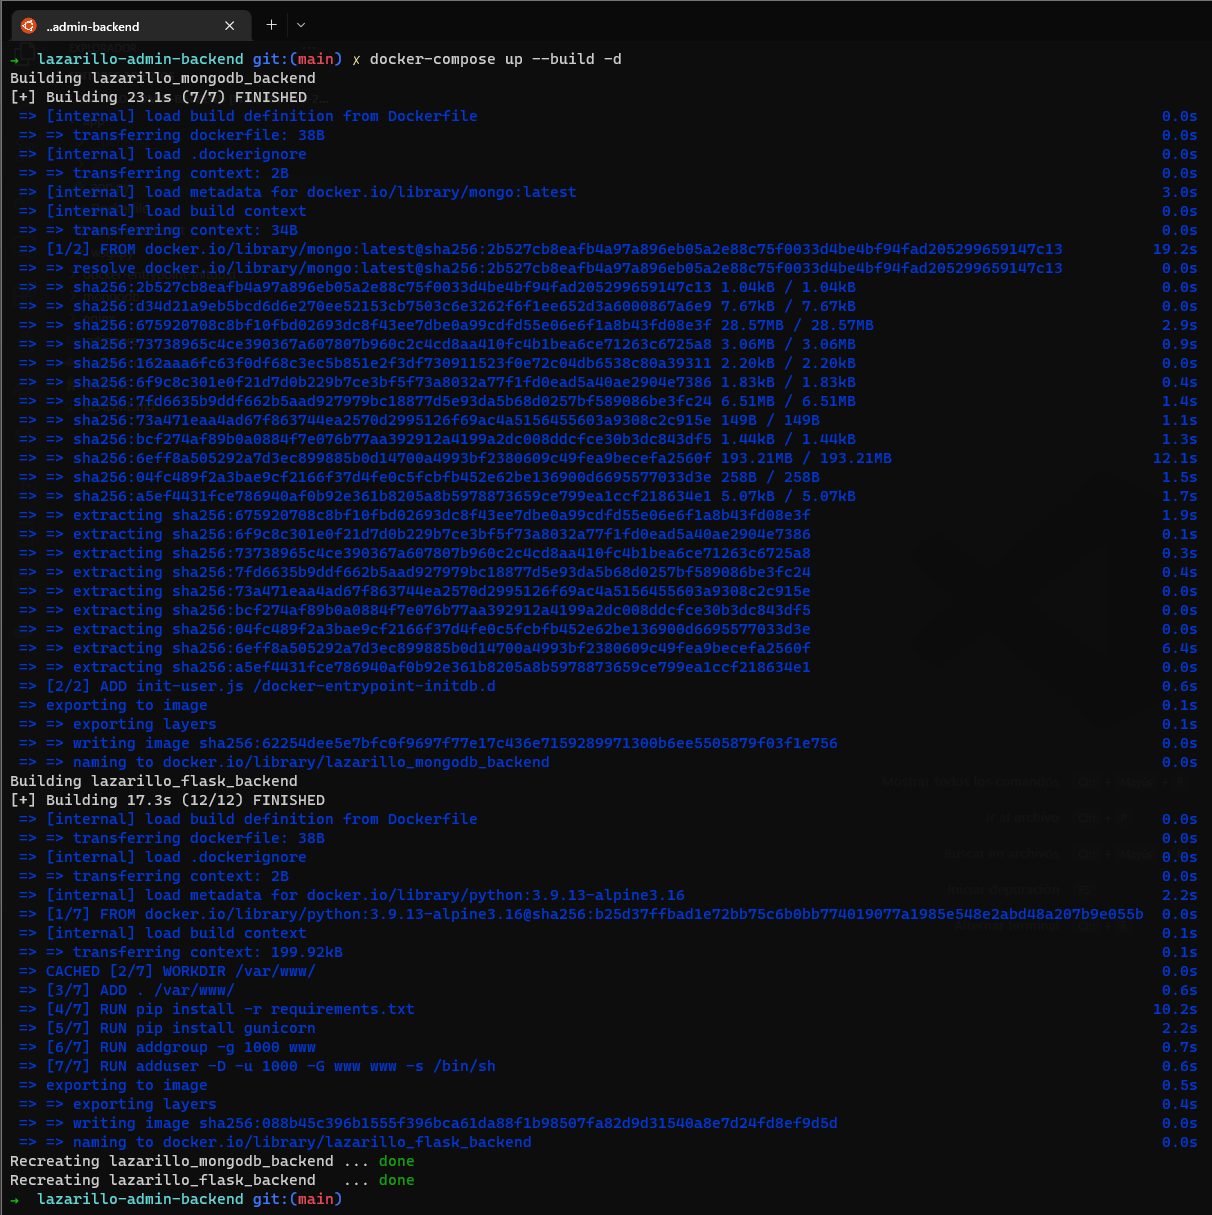
\includegraphics[width=0.75\textwidth]{imagenes/docker-compose-build.png}
	\caption{Captura de pantalla del comando de creación y ejecución de la imagen basada en \textit{docker-compose}.}
	\label{docker-compose-build}
\end{figure}

Una vez visto esto, pasemos al código en \textit{Python} que recibe las peticiones (se obvian por ahora las funciones para explicarlas de forma más cómoda en el punto siguiente):\\

\textbf{\textit{\href{https://github.com/adrianmorente/lazarillo-admin-backend/blob/main/app/app.py}{app/app.py}}}
\begin{lstlisting}
# Create app and connect to database
application = Flask(__name__)
application.config["MONGO_URI"] = 'mongodb://' + \
	os.environ['MONGODB_USERNAME'] + ':' + os.environ['MONGODB_PASSWORD'] + \
	'@' + os.environ['MONGODB_HOSTNAME'] + \
	':27017/' + os.environ['MONGODB_DATABASE']

mongo = PyMongo(application)
db = mongo.db


# Route to listen to broadcast messages from Lazarillo devices exposing their Websocket server
@application.route("/broadcast", methods=['POST'])
def read_device_broadcast():
	# code


# Route to receive the devices that exposed their WS server
@application.route("/devices", methods=['GET'])
def send_devices():
	# code


if __name__ == "__main__":
	ENVIRONMENT_DEBUG = os.environ.get("APP_DEBUG", True)
	ENVIRONMENT_PORT = os.environ.get("APP_PORT", 5000)
	application.run(host='0.0.0.0', port=ENVIRONMENT_PORT, debug=ENVIRONMENT_DEBUG)
\end{lstlisting}

El código básicamente inicializa la conexión al servicio de base de datos utilizando las variables de entorno que habíamos configurado en el fichero \textit{docker-compose.yml} que vimos antes. Ese objeto \emph{db} se utiliza en las rutas que describiremos a continuación. Acto seguido, al final del código, se lanza la aplicación para que empiece a escuchar peticiones.\\

\subsubsection{Rutas de acceso}

La aplicación solo contempla dos rutas para recibir peticiones. La primera es \textbf{\textit{/broadcast}} y solo acepta el método \textbf{\textit{POST}} para escribir nuevos datos. Ésta es la ruta a la que llaman los robots para exponer sus datos y dirección de conexión, implementando la mecánica que explicamos en la sección anterior.\\

\begin{lstlisting}
@application.route("/broadcast", methods=['POST'])
def read_device_broadcast():
	"""Read parameters from device and store them into db"""
	name = request.form.get('name')
	version = request.form.get('version')
	address = request.form.get('address')
	
	# add device to list of websocket servers
	db.devices.insert_one({
		'name': name,
		'version': version,
		'address': address
	})
	return jsonify(message='success'), 201
\end{lstlisting}

Al recibir una llamada a \textbf{\textit{/broadcast}}, se leen los campos ``nombre'', ``versión'' y ``dirección'' de los parámetros especificados. Estos se componen en un documento con ``\textit{clave: valor}'' y se insertan en la base de datos llamada \emph{devices} usando el objeto \textit{db} antes creado y la función \emph{insert\_one(\{\})} para escribir un documento nuevo.\\


\begin{lstlisting}
@application.route("/devices", methods=['GET'])
def send_devices():
	"""Retrieve devices from database and send them as JSON"""
	device = {}
	response = []
	
	for item in db.devices.find():
	device = {
		'id': item['_id'].__str__(),
		'name': item['name'],
		'version': item['version'],
		'address': item['address']
	}
	response.append(device)
	
	return jsonify(status=True, data=response)
\end{lstlisting}

Por otro lado, la ruta \textbf{\textit{/devices}} solo recibe métodos \textbf{\textit{GET}} para lectura. De forma inversa a la escritura, lo que se hace aquí es leer \textbf{todas las entradas} de la base de datos con el método \textbf{\textit{find()}}. Todos los documentos leídos se incluyen en un \textit{array} y se envían al solicitante.\\

En este caso el que realiza la llamada aquí es el servicio \textbf{\textit{lazarillo-admin-frontend}} y así consigue leer los robots que existen y a los que puede conectarse para su correcta gestión.\\

Para terminar, comprobamos que nuestra aplicación se está ejecutando correctamente para esperar peticiones (ahora mismo se ejecutan en la máquina local utilizando la aplicación de escritorio de \textit{Docker}), véase la figura \ref{docker-run}. Se puede apreciar que el servidor web expone el puerto \textbf{5000} para escuchar ahí las peticiones.\\

\begin{figure}[h]
	\centering
	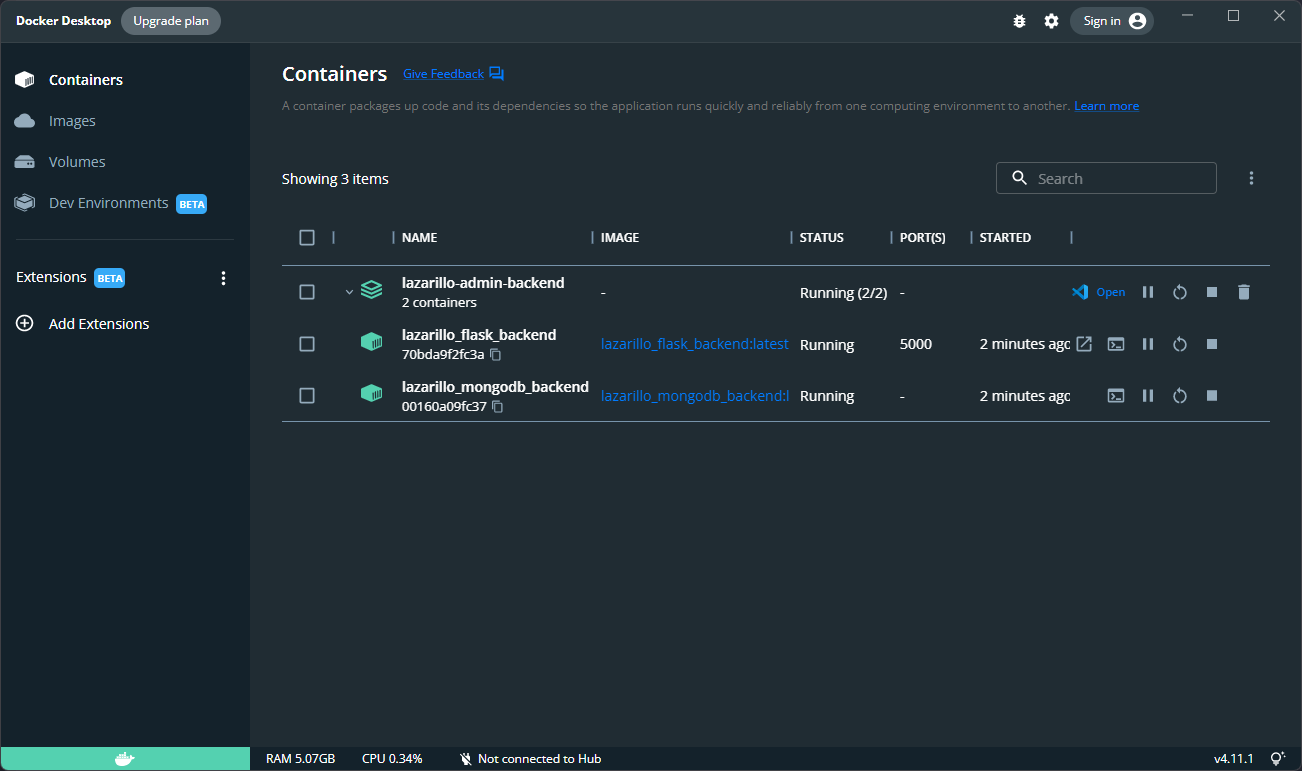
\includegraphics[width=0.75\textwidth]{imagenes/docker-run.png}
	\caption{Captura de pantalla de \textit{Docker Desktop} mostrando los dos contenedores del servidor web y la base de datos en ejecución.}
	\label{docker-run}
\end{figure}


\subsection{lazarillo-admin-frontend}











